\documentclass[a4paper,12pt,twoside]{report}

\usepackage[utf8]{inputenc}
\usepackage[english]{babel}

\usepackage{times}  
\usepackage{amsmath}
\usepackage{amssymb}
\usepackage{graphicx}
\usepackage{theorem}
\usepackage{latexsym}
\usepackage{url}
\usepackage{babel}

\headsep          0.25in
\headheight       12pt
\setlength{\topmargin}{-\headsep}
\addtolength{\topmargin}{-\headheight}
\oddsidemargin      0in
\evensidemargin     0in
\setlength{\textwidth}{\paperwidth}
\addtolength{\textwidth}{-2.0in}
\setlength{\textheight}{\paperheight}
\addtolength{\textheight}{-2.0in}
\addtolength{\textheight}{-1\topskip}
\divide\textheight  by \baselineskip
\multiply\textheight  by \baselineskip
\addtolength{\textheight}{\topskip}

\renewcommand{\contentsname}
{Table of contents}

\begin{document}

\pagestyle{plain}

%----------------------------- Front matter of the document

\title{Smoothed Particle Hydrodynamics in Zero Gravity}
\author{Oscar Westberg, Teodor Vik, Mikael Zackrisson, Anton Österblad}
\maketitle

\thispagestyle{empty}
\newpage{}

\setcounter{page}{2}
\begin{abstract}
This project was part of the course TNM085, Modeling project at Linköping University. Groups were able to choose their own research topics and simulate a physical model. This report describes a simulation of a system using Smoothed Particle Hydrodynamics (SPH) in both zero gravity and under the effect of gravity. \\

\noindent The results of the project show a way to simulate a fluid in real time using Navier-Stokes equation in C++ and OpenGL.
\vfill
\end{abstract}
\newpage{}

\tableofcontents  % chapter with the table of contents
\addtocontents{toc}{\protect\thispagestyle{empty}}
\listoffigures    % chapter with the list of figures
\addtocontents{lof}{\protect\thispagestyle{empty}}
%\listoftables     % chapter with the list of tables
%\addtocontents{lot}{\protect\thispagestyle{empty}}


%----------------------------- Body of the document

\chapter{Introduction}

%----------------------------- Background
\section{Background}
Fluid simulation is a popular tool in computer graphics and it is often used to simulate liquid, smoke and explosions. Depending on the quality requirements fluid simulations can be extremely time-consuming animations or simple real-time particle systems. Since particle system is a good way to simulate a complex effect it is very popular amongst developers and thus there are a lot of information to find about the subject. The report is based on Smoothed Particle Hydrodynamics, which is one of the most popular techniques when creating a fluid.

%----------------------------- Purpose
\section{Purpose}
The purpose of this project is to, based on mathematical models and physical formulas, perform a simulation of water in both earth like conditions and in zero gravity. The simulation shall be displayed graphically in real-time.



%----------------------------- Physical systems
\chapter{Physical systems}
There are several techniques for simulating a fluid. The most common techniques are based on the Navier-Stokes equations which describes the flow of fluids. To practically use the Navier-Stokes equations it is common to make some simplifications in which some properties are assumed to be constant. There are two fundamental approaches on how to implement the Navier-Stokes equations; the Eulerian method and the Lagrangian method. Both are widely used in computer graphics. \\

\noindent The Eulerian method uses a grid-based system, in which each grid point has fluid properties, like velocity, density, pressure, etc., but the points never move.
The Lagrangian method is based on a collection of particles that, in addition to the fluid properties, has a position and can move.

%----------------------------- Navier-Stokes
\section{Navier-Stokes equations}

Navier-Stokes

\begin{equation}
\frac{\partial \overrightarrow v}{\partial t} + ({\overrightarrow v}\cdot{\overrightarrow \nabla}){\overrightarrow v} = \frac{-\overrightarrow \nabla p}{\rho_m} + \frac{\mu}{\rho_m}{ \nabla^2}{\overrightarrow v} + \frac{\overrightarrow f_{ext}}{\rho_m}
\label{e1}
\end{equation} \\

\noindent$\rho_m$ = mass density\\*
$v$ = velocity\\*
$\nabla$= gradient\\*
$p$ = pressure\\*
$f_{ext}$ = external force\\*
$\mu$ = viscosity\\*

\noindent Navier-Stokes equations describe the motion of fluid substances as a result of forces. The forces are based on the physical quantities of the fluid (velocity v, mass density p and pressure) and also viscosity and external forces. Equation \ref{e1} describes the conservation of momentum, and basically it is Newton’s second law for a fluid.\\

%----------------------------- SPH
\section{Smoothed Particle Hydrodynamics}
Smoothed Particle Hydrodynamics (SPH) is a Lagrangian method that divides the fluid into a set of particles. Mass-density, pressure, etc. are estimated using SPH approximations. The properties of a SPH-particle is affected by other particles that lie within a certain “smoothing” distance, thus affected only by its neighbours. Any desired scalar quantity can be determined for each particle by weighting that quantity from neighboring particles with a “kernel function”. \\

\noindent SPH
\begin{equation}
{A_i} = {\sum_j A_j} \frac{m_j}{p_j} {W(r_{ij},h)}
\label{e2}
\end{equation}\\


\noindent Pressure Gradient
\begin{equation}
{-\nabla p_i} =  {-\sum_j}{m_j}\frac{p_i + p_j}{2p_j}{\nabla W(r_{ij},h)}
\label{e3}
\end{equation}

\noindent where $p_i$ and $p_j$ are pressure given by $p_i = k(p_i - p_0)$ with $p_0$ the ideal density of the fluid and $k$ a stiffness constant.\\

\noindent Viscosity
\begin{equation}
{\mu \nabla^2 \cdot v_i} = {\mu}{\sum_j}{m_j}\frac{v_j - v_i}{p_j}{\nabla^2 W(r_{ij},h)}
\label{e4}
\end{equation}



%----------------------------- Implementation
\chapter{Implementation}
An SPH simulation involves repeating these steps as time advances:
\begin{enumerate}
\item Compute density at each particle.
\item Compute pressure from density.
\item Compute forces from pressure gradients.
\item Compute external forces.
\item Apply those forces to move particles.
\end{enumerate}

%----------------------------- Matlab
\section{Matlab}
A simple version of the model was simulated in MATLAB in order to test the theory behind the system as this eliminated the chances of any potential errors being caused by the rendering or implemented functions. The calculations was performed in the order that was previously described.

%----------------------------- OpenGL
\section{OpenGL}
The particle system’s functionality was tested in MATLAB, however the final product was created in C++. The program uses the libraries glm, glew, glfw, OpenGL and standard C++ functionality to render and simulate the particle system. From the main loop the program first checks for input, then updates the particle’s properties and then render the scene mainly by using a fragment shader. \\

\noindent Since only the closest neighbors of each particle will have an effect on its behavior it’s unnecessary to calculate the effect on every particle for each particle. This gives $N^2$ calculations. The performance was improved by using spatial subdivision. A uniform grid subdivides the simulation space into a grid of uniformly sized cells. This means that the the force for a given particle can be calculated by only comparing it with all its neighbors within a certain radius. \\

\noindent To ensure the rendered scene looks like water instead of a collections of dots the technique metaballs was implemented. A metaball emits an electric field according to the formula: $[f(x,y) = 1.0 / (x^2 + y^2)]$ \\

\noindent  If the accumulated contribution of several metaball fields reaches a certain threshold, the shader renders the color blue. The metaball technique makes the entire particle system look like a fluid.



%----------------------------- Result
\chapter{Result}
The end product is an interactive program simulating a customizable amount of particles in either zero gravity or with gravity. The particle system is rendered in 2D in a window.

\begin{figure}[h]
\begin{center}
    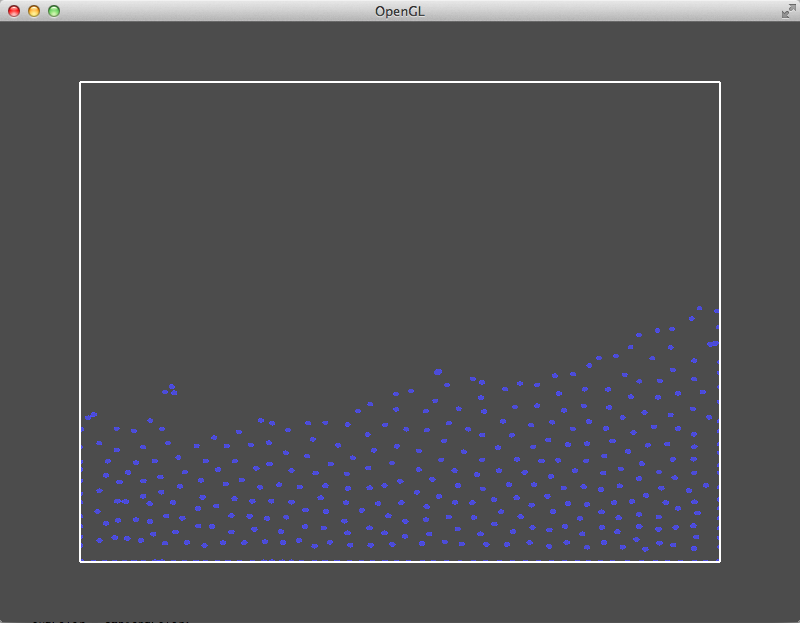
\includegraphics[width=11cm]{figs/image_2.png} 
\end{center}
\caption{Running the program without metaballs activated}
\label{model_block}
\end{figure}

\newpage{}

\begin{figure}[t]
\begin{center}
    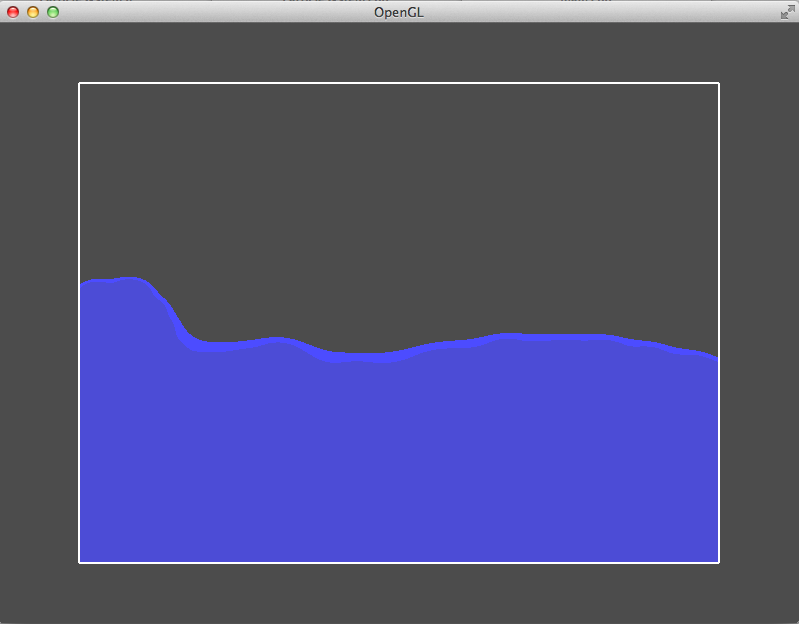
\includegraphics[width=11cm]{figs/image_1.png} 
\end{center}
\caption{Running the program with metaballs}
\label{model_block}
\end{figure}



%----------------------------- Conclusion and discussion
\chapter{Conclusion and Discussion}
...\\* \\*
Also include:\\*
Attachments\\*
Description of software and hardware requirements\\*
Manual of how to run the program



%----------------------------- Back matter of the document

\bibliographystyle{vancouver}
\bibliography{refs/references}

%\addcontentsline{toc}{chapter}{References}

%\pagestyle{empty}

%\appendix

%\cite{auer08}
%\cite{kelager06}

\begin{thebibliography}{11}

\bibitem{auer08}
  Auer, S.
  \emph{Realtime Particle-Based Fluid Simulation}.
  Computer Graphics and Visualization,
  October 4th,
  2008.
  
  \bibitem{kelager06}
  Kelager, M.
  \emph{Lagrangian Fluid Dynamics Using Smoothed Particle Hydrodynamics}.
  Department of Computer Science, University of Copenhagen,
  January 9th,
  2006.

\end{thebibliography}


\end{document}